%======================================================================
% T19_grandcanon.pdf
%======================================================================
\section{Cvičení: Grandkanonický soubor}
\strana{T19-1}

\begin{priklad}[Zadání]
\begin{enumerate}[label=\arabic*)]
  \item Ukažte, že v GK souboru platí \ $\langle(\Delta N)^2\rangle = Nk_BT\dfrac{\kappa_T}{v}$
        \quad \textcolor{NavyBlue}{-- viz hlavní poznámky}
  \item GK popis id.\ plynu
  \begin{enumerate}[label=\arabic*)]
    \item najděte $Z_G(\beta,V,\alpha)$ a $\Phi(T,V,\mu)$
    \item odvoďte termickou a kalorickou stavovou rovnici $p = p(T,V,N)$ \& $E = E(T,V,N)$
    \item najděte chem.\ potenciál $\mu = \mu(T,V,N)$ a diskutujte jeho znaménko
    \item najděte fluktuace počtu částic a energie
  \end{enumerate}
  \item[3)$^*$] Ideální plyn v gravitačním poli
  \begin{enumerate}[label=\arabic*)]
    \item najděte \uv{barometrickou formuli} $p = p(T,N,z)$
  \end{enumerate}
\end{enumerate}
\end{priklad}

\noindent\rule{\linewidth}{0.4pt}

\begin{veta}[Kuchařka pro GK soubor]
\begin{enumerate}[label=\arabic*),leftmargin=3.5em]
  \item[1) \& 2)] viz kanonický: \quad
        $Z_c^{(N)} = \displaystyle\int\dd\Gamma_N\,e^{-\beta H} \overset{\substack{\text{pro nezáv.\ st.\ volnosti /}\\ \text{částice}}}{=} \textcolor{NavyBlue}{\frac{1}{N!}}(Z_1)^N$
        \quad \textcolor{NavyBlue}{$\nwarrow$ může a nemusí být}
  \item[3)] $Z_G = \displaystyle\sum_N Z_c^{(N)}e^{\alpha N} = \exp\big(e^\alpha Z_1\big)$ \quad
        $\big(\uparrow\ Z_c^{(N)} = \frac{1}{N!}Z_1^N\big)$
        \begin{itemize}[nosep]
          \item jiný častý trik: \quad $Z_G = \displaystyle\sum_{N=0}^{M}\binom MN Z_1^Ne^{\alpha N} = \big(1 + Z_1e^\alpha\big)^M$
        \end{itemize}
  \item[4)] $\Phi(T,V,\mu) = -\dfrac1\beta\log Z_G(\beta,V,\alpha = \beta\mu)\Big/_{\beta = \frac{1}{k_BT}}$ \quad $\Rightarrow$ termodynamika \dots
  \item[5)] Nakonec často \ $\langle N\rangle = -\dfrac{\partial\Phi}{\partial\mu}$ \ \& dosazení $\mu = \mu(T,V,\langle N\rangle)$ \\
        \hspace*{4cm}$\big[$resp.\ $e^{\beta\mu} = e^\alpha = e^\alpha(T,V,\langle N\rangle)\big]$
\end{enumerate}
\end{veta}

%----------------------------------------------------------------------
\strana{T19-2}
{\color{NavyBlue}
\subsection*{2) GK popis id.\ plynu}
\[
  Z_G = \sum_N Z_c^{(N)}e^{\alpha N}
\]
$\bullet$ kanonická part.\ funkce: \ $Z_c^{(N)} = \dfrac{1}{N!}(Z_1)^N$ \dots\ viz minule
\[
  Z_1 = V\Big(\frac{2\pi m}{h^2\beta}\Big)^{3/2} = V\lambda_T^{-3}
\]
\quad NB: de Broglie termální vlnová délka \quad
$\lambda_T = \sqrt{\dfrac{2\pi\hbar^2}{mk_BT}} = \sqrt{\dfrac{h^2\beta}{2\pi m}}$
\[
  \Rightarrow\ Z_G = \sum_{N=0}^{\infty}\frac{1}{N!}\big(V\lambda_T^{-3}e^\alpha\big)^N = \exp\big(V\lambda_T^{-3}e^\alpha\big)
  \qquad \textcolor{Red}{\text{NB: nepotřebuji Stirlinga!}}
\]
\[
  \Rightarrow\ \Phi(T,V,\mu) = -k_BT\log Z_G = -k_BTV\lambda_T^{-3}e^\alpha
  \qquad \alpha = \beta\mu = \frac{\mu}{k_BT} \qquad \lambda_T = \Big(\frac{2\pi\hbar^2}{mk_BT}\Big)^{1/2}
\]
\[
  \Rightarrow\ \vzorec{\Phi(T,V,\mu) = -k_B\Big(\frac{mk_B}{2\pi\hbar^2}\Big)^{3/2}VT^{5/2}e^{\frac{\mu}{k_BT}}}
  \qquad \dd\Phi = -S\,\dd T - p\,\dd V - N\,\dd\mu
\]
\[
  \bullet\ \langle N\rangle = -\frac{\partial\Phi}{\partial\mu} = \Big(\frac{mk_B}{2\pi\hbar^2}\Big)^{3/2}VT^{3/2}e^{\frac{\mu}{k_BT}}
  = -\frac{\Phi}{k_BT}
\]
$\Rightarrow$ 1) \ $\Phi = -pV$ pro jednoduchý plyn \\
\hspace*{1.2cm}$\Rightarrow$ dostáváme \uv{správnou} stavovou rci \quad $\langle N\rangle k_BT = pV$ \ $\checkmark$

\phantom{$\Rightarrow$} 2) \
$\langle E\rangle = -\dfrac{\partial}{\partial\beta}\log Z_G = -Ve^\alpha\dfrac{\partial}{\partial\beta}\Big(\dfrac{h^2\beta}{2\pi m}\Big)^{-3/2}$ \\[3pt]
\hspace*{2.3cm}$= \dfrac32Ve^\alpha\Big(\dfrac{h^2\beta}{2\pi m}\Big)^{-3/2}\beta^{-1} = -\dfrac32\Phi = \dfrac32pV = \dfrac32\langle N\rangle k_BT$ \ $\checkmark$
}

%----------------------------------------------------------------------
\strana{T19-3}
{\color{NavyBlue}
3) \ $\langle N\rangle = V\lambda_T^{-3}e^{\frac{\mu}{k_BT}} \Rightarrow e^{\frac{\mu}{k_BT}} = \dfrac NV\lambda_T^3$
\[
  \Rightarrow\ \vzorec{\mu = k_BT\log\Big(\frac NV\lambda_T^3\Big)}
\]
\begin{enumerate}[label=\alph*)]
  \item dostáváme absolutní hodnotu $\mu$ \\
        -- kanonický soubor dává také $\mu$ bez volných konstant -- je stejné? (DCv)
  \item $\dfrac VN = v = d^3$ \quad $d$ \dots\ char.\ vzdálenost mezi částicemi
        \[ \Rightarrow\ \text{pro } d > \lambda_T \text{ je } \text{\pozor{$\mu < 0\,!$}} \]
        $\mu = \Big(\dfrac{\partial E}{\partial N}\Big)_{S,V}$ \dots\ důležitá pro vysvětlení je ona konst.\ entropie: energie systému s novou
        částicí vzroste o její kin.\ energii; vzroste ovšem také entropie $\Rightarrow$ pro udržení její konstantnosti je třeba odčerpat
        teplo $\Leftrightarrow$ snížit střední kin.\ energii částic \\
        \hspace*{2cm}\dots\ $\mu < 0$ znamená, že tohoto tepla je víc než energie, kterou přinesla nová částice
  \item $d \lesssim \lambda_T \Rightarrow$ přestává platit klasická fyzika (příliš hustý plyn nebo příliš nízká teplota)
        $\Rightarrow$ chem.\ potenciál id.\ plynu je záporný nebo model nefunguje
\end{enumerate}

4) \ $\langle(\Delta N)^2\rangle = \dfrac{\partial^2\log Z_G}{\partial\alpha^2} = V\lambda_T^{-3}e^\alpha = \langle N\rangle$
\[
  \overset{\text{(obecně)}}{=}\ Nk_BT\frac{\kappa_T}{v} \ \Rightarrow\ \kappa_T = \frac{v}{k_BT}
\]
\underline{ověřme:} \ $\kappa_T = -\dfrac1v\Big(\dfrac{\partial v}{\partial p}\Big)_T = \Big/\,v = \dfrac{k_BT}{p}\Big/ = \dfrac1v\dfrac{k_BT}{p^2} = \dfrac1p = \dfrac{v}{k_BT}$ \ $\checkmark$
}

%----------------------------------------------------------------------
\strana{T19-4}
{\color{NavyBlue}
\begin{align*}
  \langle(\Delta E)^2\rangle &= \frac{\partial^2\log Z}{\partial\beta^2} = -\frac{\partial\langle E\rangle}{\partial\beta}
   = -\frac{\partial}{\partial\beta}\frac32Ve^\alpha\Big(\frac{h^2}{2\pi m}\Big)^{-3/2}\beta^{-5/2} \\
  &= \frac{15}{4}Ve^\alpha\Big(\frac{h^2}{2\pi m}\Big)^{-3/2}\beta^{-7/2}
   \hspace{3cm} C_V = \tfrac32\langle N\rangle k_B \\
  &= \frac52\langle E\rangle\beta^{-1} = \frac52\underset{\substack{\uparrow\\ \frac32\langle N\rangle k_BT}}{\langle E\rangle}k_BT
   = \frac52C_Vk_BT^2 \propto N
\end{align*}
$\Rightarrow$ \ $\langle(\Delta E)^2\rangle \propto N$ podle očekávání \\
$\Rightarrow$ \ fluktuace větší než v kanon.\ souboru (přispívají fluktuace $N$)

\noindent\rule{0.85\linewidth}{0.4pt} \ DONE
}

%----------------------------------------------------------------------
\strana{T19-5}
{\color{NavyBlue}
\subsection*{3) Ideální plyn v grav.\ poli -- barometrická formule $p = p(z)$}
\begin{itemize}
  \item $H_1 = \dfrac{p^2}{2m} + mgz \ \to\ Z = \dfrac{1}{N!}(Z_1)^N$; \quad $Z_1 = \displaystyle\int\dd\Gamma_1\,e^{-\beta H_1}$
  \item minule jsme řešili kanonicky a dospěli jsme ke vztahu pro \uv{volnou energii}
        \[
          F = F(\underset{\text{plocha \uv{podstavy}}}{T,\Sigma},N,\underset{\substack{\uparrow\\ \text{grav.\ síla} \equiv \text{síla sdružená k souř.\ } z}}{mg})
        \]
  \item Jak určit tlak? \pozor{Nelze!} V tomto popisu \underline{není dobře def.} Intuitivně chápeme, že \uv{lokálně} měřený tlak závisí
        na $\underline z$, není tedy stejný v celém objemu, jak jsme v TD v rovnovážném stavu vždy požadovali od intenzivních proměnných.
  \item \underline{Rigorózně:}
        \[
          k_B\log Z = S\Big[\frac1T,\overset{\substack{mg\\ \swarrow}}{\frac{F_z}{T}}\Big]
          \quad\dots\ \text{nějaká podivná Massieu funkce s diferenciálem}
        \]
        \[
          \dd S[\,\cdot\,,\cdot\,] = -\underset{\substack{\uparrow\\ \langle H\rangle = U + \langle mgz\rangle = U + mg\langle z\rangle}}{E}\,\dd\Big(\frac1T\Big)
          + \frac{\hat p}{T}\,\dd\Sigma - \langle z\rangle\,\dd\Big(\frac{F_z}{T}\Big) - \frac\mu T\,\dd N
        \]
        \begin{enumerate}[label=\roman*)]
          \item Jak interpretovat $\hat p$?
          \item Přes $z$ je vyintegrováno, dostupná je již jen střední hodnota $\Rightarrow$ lokální závislost čehokoliv na $z$ je ztracena
        \end{enumerate}
\end{itemize}
$\Rightarrow$ pro nalezení $p = p(z)$ je třeba uvažovat vzájemnou rovnováhu mezi infinitezimálními \uv{vrstvami plynu}
$\Rightarrow$ ideální bude GK soubor, neboť vrstvy mohou vyměňovat částice
\begin{itemize}
  \item vrstvy lze popisovat i kanonicky, ale je to nešikovné
\end{itemize}}

%----------------------------------------------------------------------
\strana{T19-6}
{\color{NavyBlue}
\underline{Řešení}

\begin{minipage}{0.48\textwidth}
\begin{enumerate}[label=\arabic*)]
  \item najdeme velký potenciál $\Phi$ pro 1 vrstvu jako funkci $z$
  \item vrstvy jsou v tepelné a chem.\ rovnováze
  \begin{enumerate}[label=\roman*)]
    \item $\beta(z) = \beta(z + \delta z) \Leftrightarrow \beta = \text{konst}$
    \item $\mu(z) = \mu(z + \delta z) \Leftrightarrow \mu = \text{konst}$
  \end{enumerate}
\end{enumerate}
\end{minipage}
\begin{minipage}{0.5\textwidth}
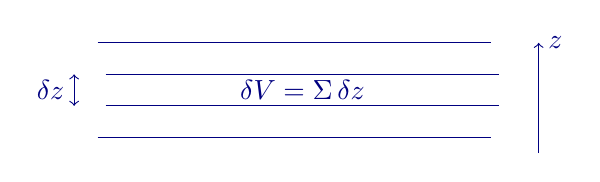
\begin{tikzpicture}[NavyBlue]
  \draw (0,1.6) -- (5,1.6);
  \draw (0.1,1.2) -- (5.1,1.2);
  \draw (0.1,0.8) -- (5.1,0.8);
  \draw (0,0.4) -- (5,0.4);
  \node at (2.6,1.0) {$\delta V = \Sigma\,\delta z$};
  \draw[<->] (-0.3,0.8) -- (-0.3,1.2) node[midway,left] {$\delta z$};
  \draw[->] (5.6,0.2) -- (5.6,1.6) node[right] {$z$};
\end{tikzpicture}
\end{minipage}

\begin{enumerate}[label=\arabic*),start=3]
  \item $\dd\Phi(T,\delta V,\mu,z) = \dots - p\,\dd(\delta V)\dots$ \\
        $\Rightarrow$ loc.\ je tlak dobře definován: \quad $p(z) = -\dfrac{\dd\Phi}{\dd(\delta V)}$
  \item hodnotu $\mu$ určíme z celkového počtu částic \\
        (typický krok při GK popisu, veličiny závislé na $\mu$ nám obvykle mnoho neřeknou)
\end{enumerate}

\noindent\rule{0.6\linewidth}{0.4pt}

ad 1) \ $\bullet$ \
$Z_1(z) = \displaystyle\int\limits_{\substack{x,y\in\Sigma\\ z\in(z\pm\delta z/2)}}\dd\Gamma_1\,e^{-\beta H_1}
 = \frac{\Sigma\,\delta z}{h^3}e^{-\beta mgz}\int\dd^3p\,e^{-\beta\frac{p^2}{2m}}$
\quad \small($\Rightarrow$ $z$ v int.\ mohu brát konst.)\normalsize
\[
  \Rightarrow\ Z_1 = \frac{\delta V}{h^3}e^{-\beta mgz}\Big(\frac{2\pi m}{\beta}\Big)^{3/2}
\]
$\bullet$ \
$Z_G = \displaystyle\sum_{\delta N}\frac{1}{(\delta N)!}(Z_1)^{\delta N}e^{\alpha\delta N}
 = \exp\Big(\frac{\delta V}{h^3}e^{\alpha - \beta mgz}\Big(\frac{2\pi m}{\beta}\Big)^{3/2}\Big)$ \\
\hspace*{1cm}$\uparrow$ $\delta N$ je \#částic v dané vrstvě

$\bullet$ \
$\Phi = -\dfrac1\beta\log Z_G = -\dfrac{\delta V}{h^3}\overset{\substack{\alpha = \beta\mu\\ \swarrow}}{e^{\beta\mu}}e^{-\beta mgz}(2\pi m)^{3/2}\beta^{-5/2}$
}

%----------------------------------------------------------------------
\strana{T19-7}
{\color{NavyBlue}
\underline{Pozn:}
\begin{itemize}[nosep]
  \item striktně vzato bych měl nahradit $\beta = \frac{1}{k_BT}$, ale tady to úplně nevadí, protože $T\Leftrightarrow\beta$ bude stále
        konst.; důležité je nemíchat $T$ \& $\beta$
  \item důležité je $\alpha\to\beta\mu$, abych \uv{nepřehlédl} tuto závislost na $\beta$
\end{itemize}

ad 2) \ už mám vlastně vyřešeno, $\mu$ \& $\beta$ jsou konst.\ nezávislé na $z$

ad 3) \ $\Phi = \Phi(\beta,\delta V,\mu;\underline{z,mg})$ \\
\hspace*{4cm}$\uparrow$ nejsou v tomto popisu TD parametry v klas.\ smyslu toho \uv{pojmu}
\[
  \Rightarrow\ p(\beta,\delta V,\mu;z,mg) = -\frac{\dd\Phi}{\dd(\delta V)}
  = \frac{1}{h^3}e^{\beta\mu}e^{-\beta mgz}(2\pi m)^{3/2}\beta^{-5/2} = -\frac{\Phi}{\delta V} \qquad (*)
\]

ad 4) \ tato formule opravdu není příliš užitečná \\
\quad $\Rightarrow$ $e^{\beta\mu}$ určíme takto:
\begin{enumerate}[label=\roman*)]
  \item $\langle\delta N\rangle(z,\mu) = -\dfrac{\partial\Phi}{\partial\mu}$ \quad $\Big(= \dfrac{\partial\log Z_G}{\partial\alpha}\Big)$
  \item $N = \displaystyle\int\langle\delta N\rangle$
\end{enumerate}
$\bullet$ \ $\langle\delta N\rangle = -\dfrac{\partial\Phi}{\partial\mu} = -\beta\Phi \overset{(*)}{=} \beta p\,\delta V$
\ $\Rightarrow$ nepřekvapivě dostáváme stav.\ rovnici id.\ plynu
}

%----------------------------------------------------------------------
\strana{T19-8}
{\color{NavyBlue}
\[
  N = \int\langle\delta N\rangle = \int_0^\infty\dd z\,\frac{\Sigma}{h^3}e^{\beta\mu}e^{-\beta mgz}(2\pi m)^{3/2}\beta^{-3/2}
\]
\hspace*{2.5cm}$\uparrow$ $\langle\delta N\rangle \propto \delta V = \Sigma\,\dd z \Rightarrow \int\langle\delta N\rangle = \int_0^\infty\bullet\,\dd z$
\[
  = \frac{\Sigma e^{\beta\mu}}{h^3}\Big(\frac{2\pi m}{\beta}\Big)^{3/2}\frac{e^{-\beta mgz}}{\beta mg}\Big|_\infty^0
  = \frac{\Sigma e^{\beta\mu}}{mgh^3}(2\pi m)^{3/2}\beta^{-5/2}
\]
\[
  \Rightarrow\ e^{\beta\mu} = \frac N\Sigma\,\frac{mgh^3}{(2\pi m)^{3/2}}\,\beta^{5/2}
\]
$\bullet$ \ $p = \dfrac{1}{h^3}e^{\beta\mu}e^{-\beta mgz}(2\pi m)^{3/2}\beta^{-5/2} = \dfrac N\Sigma\,mg\,e^{-\beta mgz}$

$\bullet$ \ protože ale ani $N$ neznáme, spokojíme se s klasickým výsledkem
\[
  \vzorec{p = p_0\,e^{-\frac{mgz}{k_BT}}}
\]
\hfill\rule{0.45\linewidth}{0.4pt} \ DONE
}
